\chapter{Appendice B}
L'interfaccia grafica � una componente importante per quanto riguarda l'interazione con il software. Nel caso di NNSec, questa si suddivide in due componenti e mette a disposizione lato server un metodo per configurare il sistema e caricare nuove reti neurali in modo da metterle a disposizione di utenti remoti, mentre per i client sono disponibili controlli veloci ed intuitivi per il recupero della lista di reti neurali disponibili e l'uso di quest'ultime. Inoltre, in entrambi i casi � presente un'area di log in cui sono riportati dati utili o informazioni sommarie in caso di eventuali errori.\\
Brevemente, saranno descritte nel seguito le interfacce grafiche lato client e lato server e come queste possono essere utilizzate per interagire con NNSec a seconda dei casi.

\paragraph{Interfaccia lato client.}
Per quanto riguarda il client, l'interfaccia grafica � concepita per permette all'utente una connessione remota verso un server NNSec, il recupero della lista di reti neurali disponibili su di esso e quindi l'uso di quest'ultime.\\
\begin{figure}[ht]
\centering
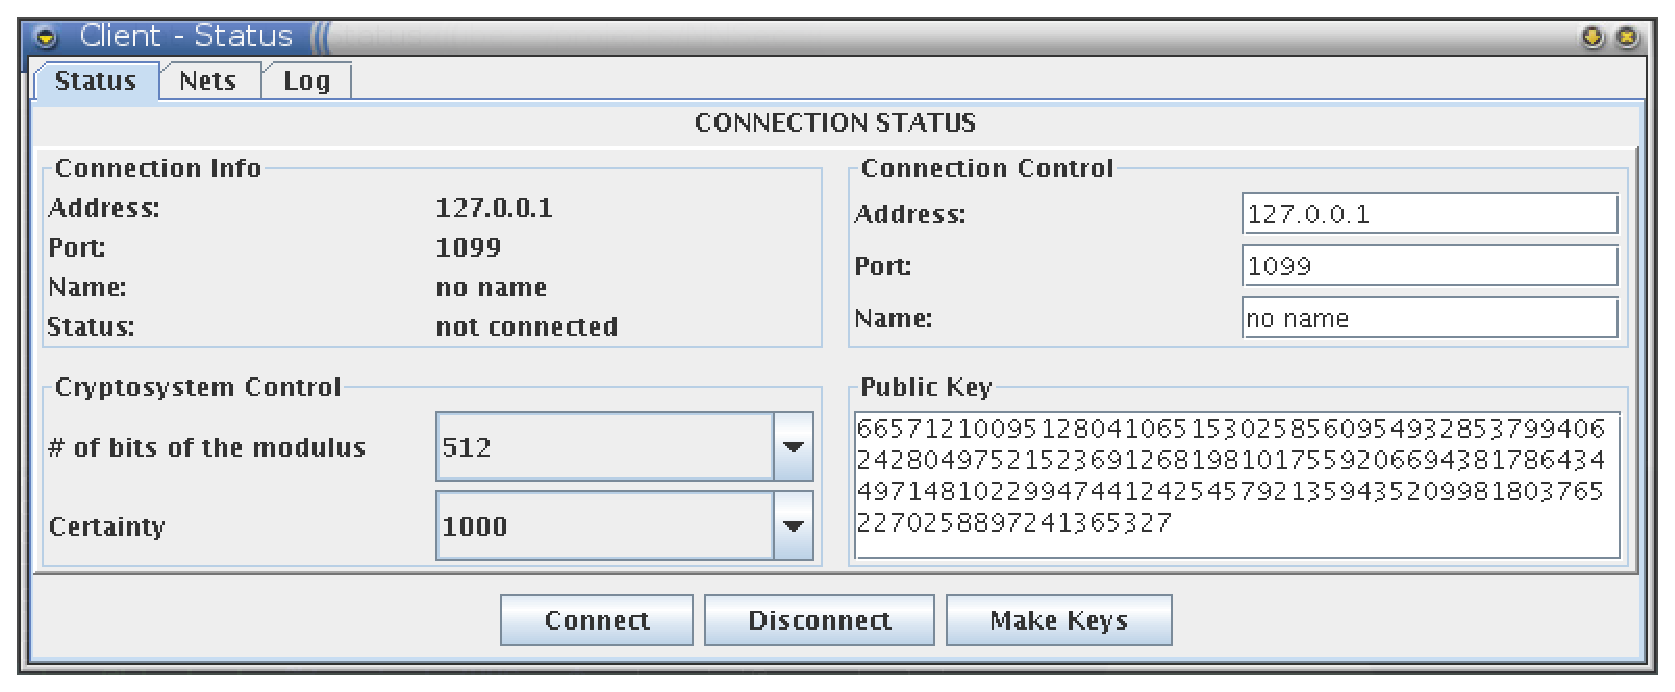
\includegraphics[scale=0.45]{img/cstat.eps}
\end{figure}
Tramite il pannello \textit{status} � possibile indicare l'indirizzo IP del server desiderato e quindi la porta su cui effettuare la connessione, oltre al nome del server che si vuole contattare. Nello stesso pannello sono riportati dati riguardanti la connessione stessa, come ad esempio il fatto che essa sia attiva o meno. Ancora, dal pannello di status � possibile gestire la propria chiave pubblica impostandone a piacere i parametri e generandone di nuove ogni volta che lo si desidera, con la possibilit� di consultazione.\\
\begin{figure}[ht]
\centering
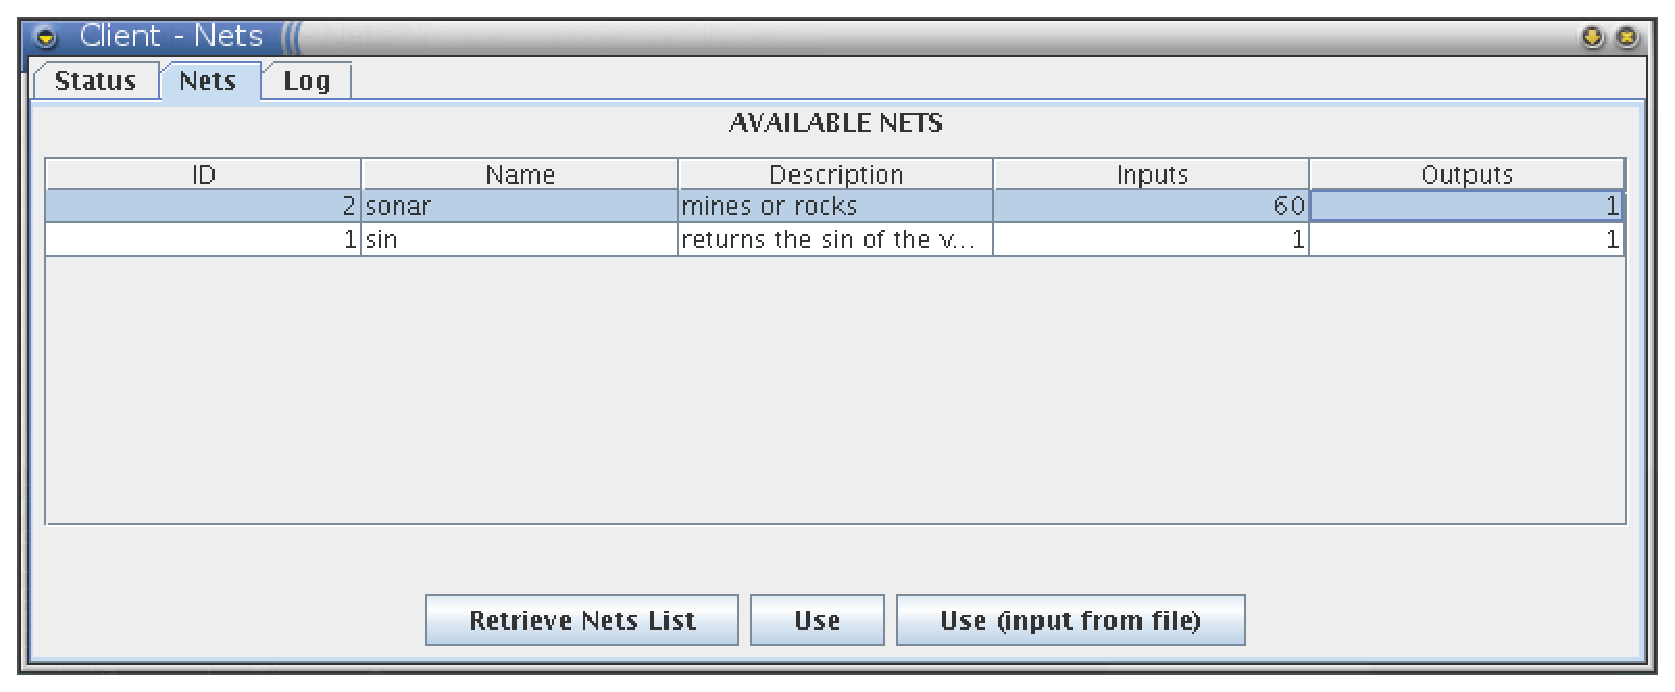
\includegraphics[scale=0.45]{img/cnets.eps}
\end{figure}
Dal pannello \textit{Nets} si pu� procedere al recupero e l'uso delle reti neurali. Una volta stabilita la connessione, infatti, tramite quest'area si pu� accedere alle reti neurali disponibili scaricandone una lista dal server e quindi procedere all'uso di una di queste tramite l'inserimento manuale dei dati di ingresso o, nei casi in cui questo risulta scomodo a causa della loro mole, facendo leggere i dati di ingresso direttamente da un file di ingresso sul quale questi dovranno apparire in numero di uno per riga.\\
\begin{figure}[ht]
\centering
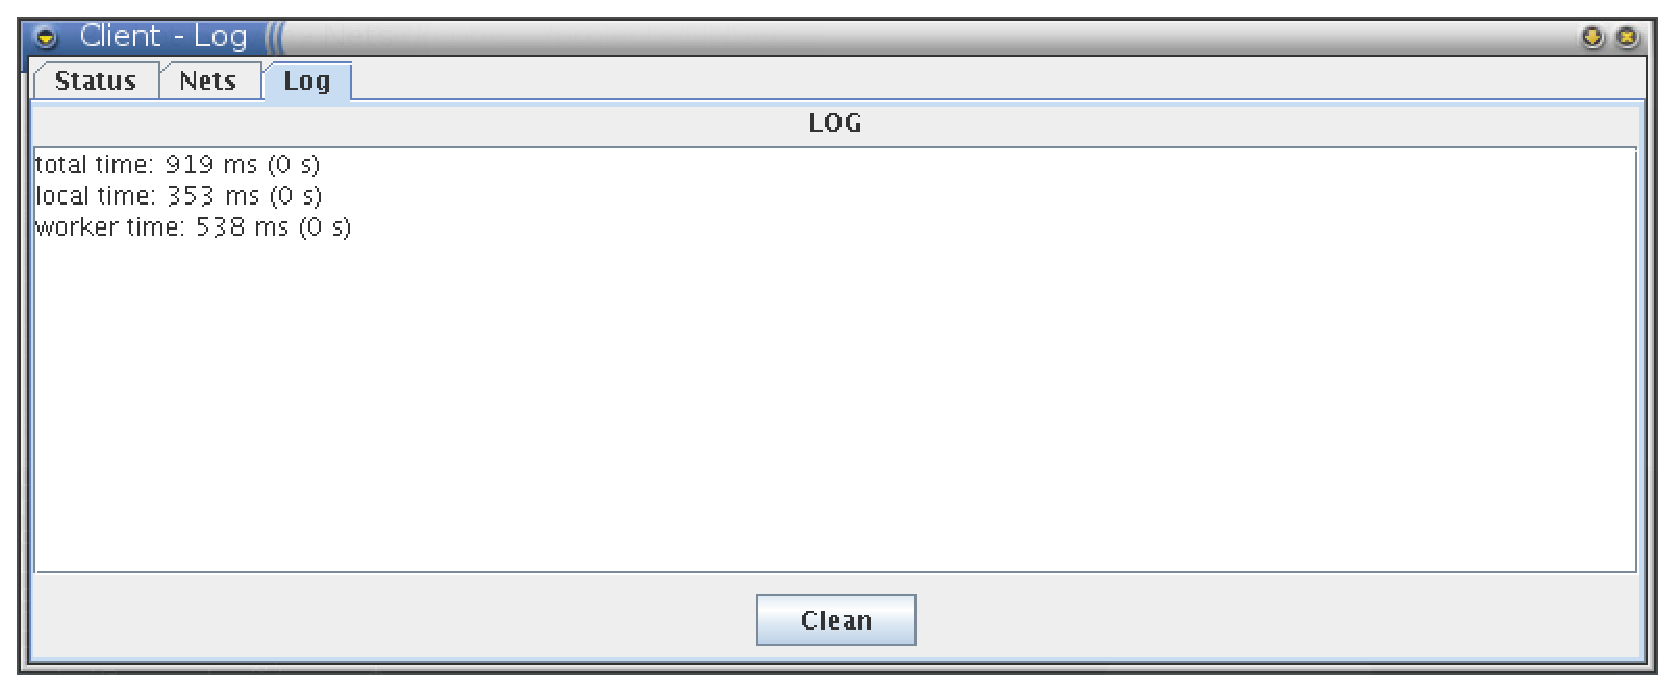
\includegraphics[scale=0.45]{img/clog.eps}
\end{figure}
In caso di errori durante la connessione ad un server o l'uso di una rete neurale, oppure addirittura in caso di errori interni al programma, nell'area di \textit{log} si pu� ottenere una breve descrizione dell'errore per cercare di capire a cosa sia dovuto il problema. Lato client, inoltre, in questa zona sono riportati dati descrittivi riguardanti la singola sessione d'uso di una rete neurale, ovvero � indicato in modo approssimativo il tempo di elaborazione totale, quello impiegato sul server e quello impiegato sul client, dai quali � poi possibile ricavare il tempo perso nelle fasi di trasmissione dei dati.

\paragraph{Interfaccia lato server.}
\begin{figure}[ht]
\centering
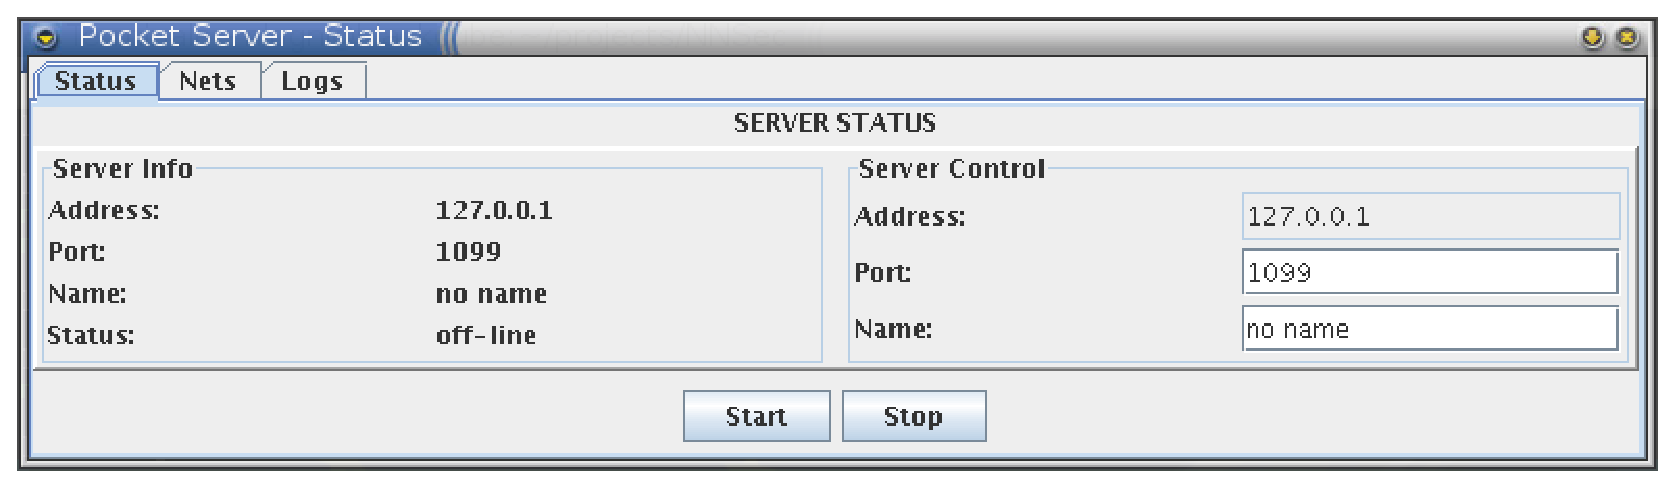
\includegraphics[scale=0.45]{img/sstat.eps}
\end{figure}
L'interfaccia grafica del server mette a disposizione metodi e campi per aggiungere nuove reti neurali al sistema, impostarne i parametri e renderle disponibili per gli utenti remoti. Questo �, senza dubbio, lo scopo primario del server e quindi deve risultare quanto pi� facile, flessibile e intuitivo possibile.\\
\begin{figure}[ht]
\centering
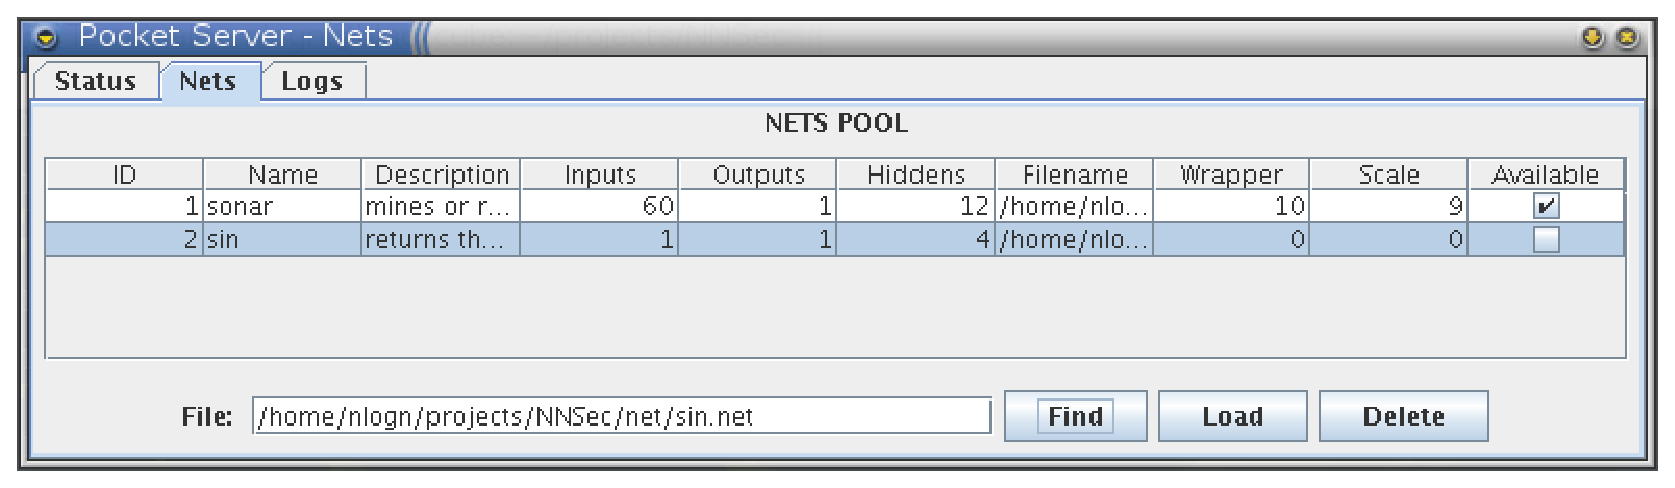
\includegraphics[scale=0.45]{img/snets.eps}
\end{figure}
Il pannello \textit{status} permette di gestire alcuni parametri relativi al server quali la porta su cui questo dovr� ascoltare e il nome a cui dovr� rispondere, in base alle chiamate. Da osservare che, in realt�, questi parametri sono relativi al registro rmi che fornir� ai client il riferimento al server NNSec (riferimento che, effettivamente, � associato al nome indicato in questo pannello). Come nel caso del pannello \textit{status} presente sul client, anche lato server sono riportati parametri relativi la connessione, come ad esempio il suo stato.\\
\begin{figure}[ht]
\centering
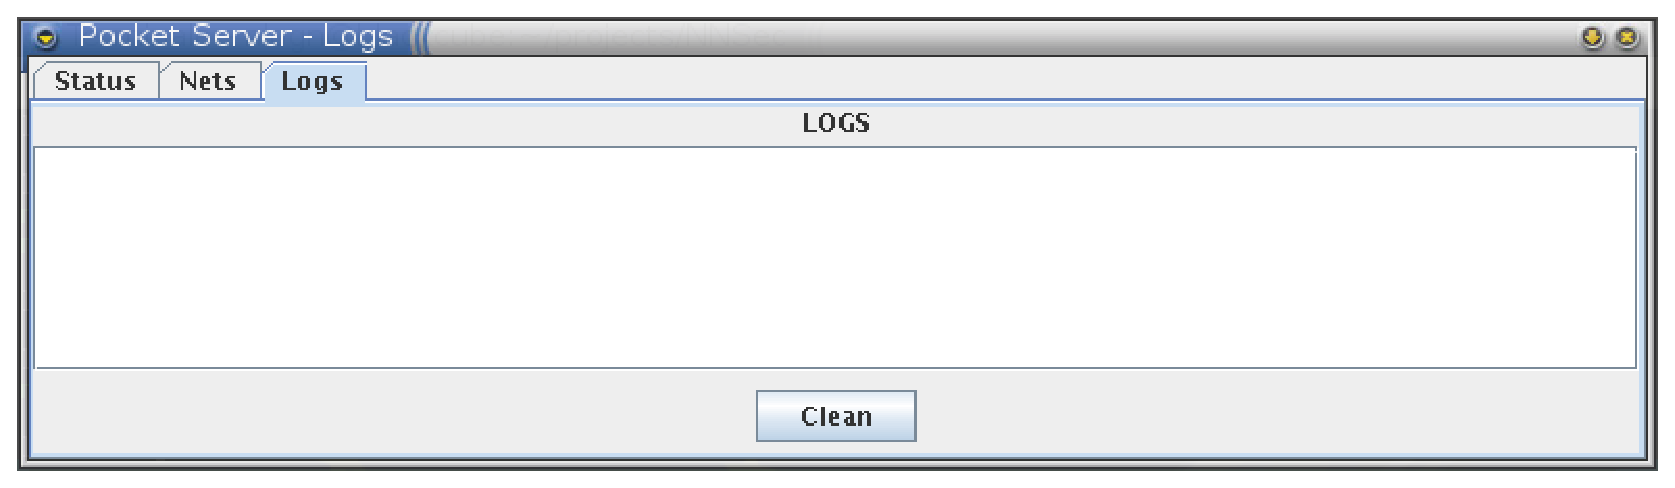
\includegraphics[scale=0.45]{img/slog.eps}
\end{figure}
Il pannello \textit{Nets} rappresenta il cuore della gestione delle reti neurali, ovvero il modo attraverso il quale l'utente pu� interagire e configurare tali elementi. Come si pu� notare � possibile caricare (ricercando sul filesystem il file di descrizione apposito) nuove reti neurali nel sistema, quindi associare ad ognuna di loro in modo indipendente un fattore di quantizzazione appropriato e il numero desiderato di nodi fittizi associati. Infine, tramite questo pannello � possibile decidere quali reti neurali risulteranno disponibili o meno agli utenti remoti.\\
Nell'area di \textit{log} sono riportati messaggi di errore interni al sistema. Esempi di queste situazioni di errore sono l'impossibilit� di effettuare il parsing dei file di descrizione per le reti neurali, l'incapacit� di creazione del registro di nomi per rmi e l'associazione quindi del riferimento locale o anche errori specifici del programma come, ad esempio, la mancanza di determinate classi laddove queste siano state cancellate per errore.
